%! Author = itgramic
%! Date = 05.12.23

% Preamble
\clearpage
\begin{flushleft}
    \subsubsection{CloudNativePG}
    CloudNativePG ist eine Containerlösung für PostgreSQL auf Kubernetes.\\
    CloudNativePG wurde ursprünglich von EDB entwickelt.
\end{flushleft}
\begin{flushleft}
    \paragraph{Core-Features}
    Die wichtigsten Features von CloudNativePG sind\cite{5ALQPE2U}:
    \begin{itemize}
        \item k8s API Integration
        \item Automatischer Failover
        \item Self-Healing von Nodes resp. Replikas
        \item Skalierbarkeit (vertikal, horizontal bedingt)
        \item Volumne Backup
        \item Object Backup
        \item Rolling PostgreSQL Upgrade / Updates
        \item Pooling mit PgBouncer
        \item Offline und Online Import von bestehenden \Gls{PostgreSQL} DBs
    \end{itemize}
\end{flushleft}
\begin{flushleft}
    \paragraph{Replikation}
    CloudNativePG bietet die üblichen PostgreSQL-Replikaionen an.
\end{flushleft}
\begin{flushleft}
    \paragraph{Proxy}
    CloudNativePG benötigt keinen zusätzlichen Proxy.
\end{flushleft}
\begin{flushleft}
    \paragraph{Pooling}
    CloudNativePG unterstützt pgBouncer als \Gls{Connection Pooler}.
\end{flushleft}
\begin{flushleft}
    \paragraph{API / Skripte}
    CloudNativePG bietet eine API zum Monitoren und Verwalten von Backups, Clustern und dem System selbst\cite{LY8V4XQM}.
\end{flushleft}
\clearpage
\begin{flushleft}
    \paragraph{Architektur}
    Kubernetes regelt die Zugriffe mit Hilfe eines entsprechenden Services in die Nodes auf den Pods:
    \begin{figure}[H]
        \centering
        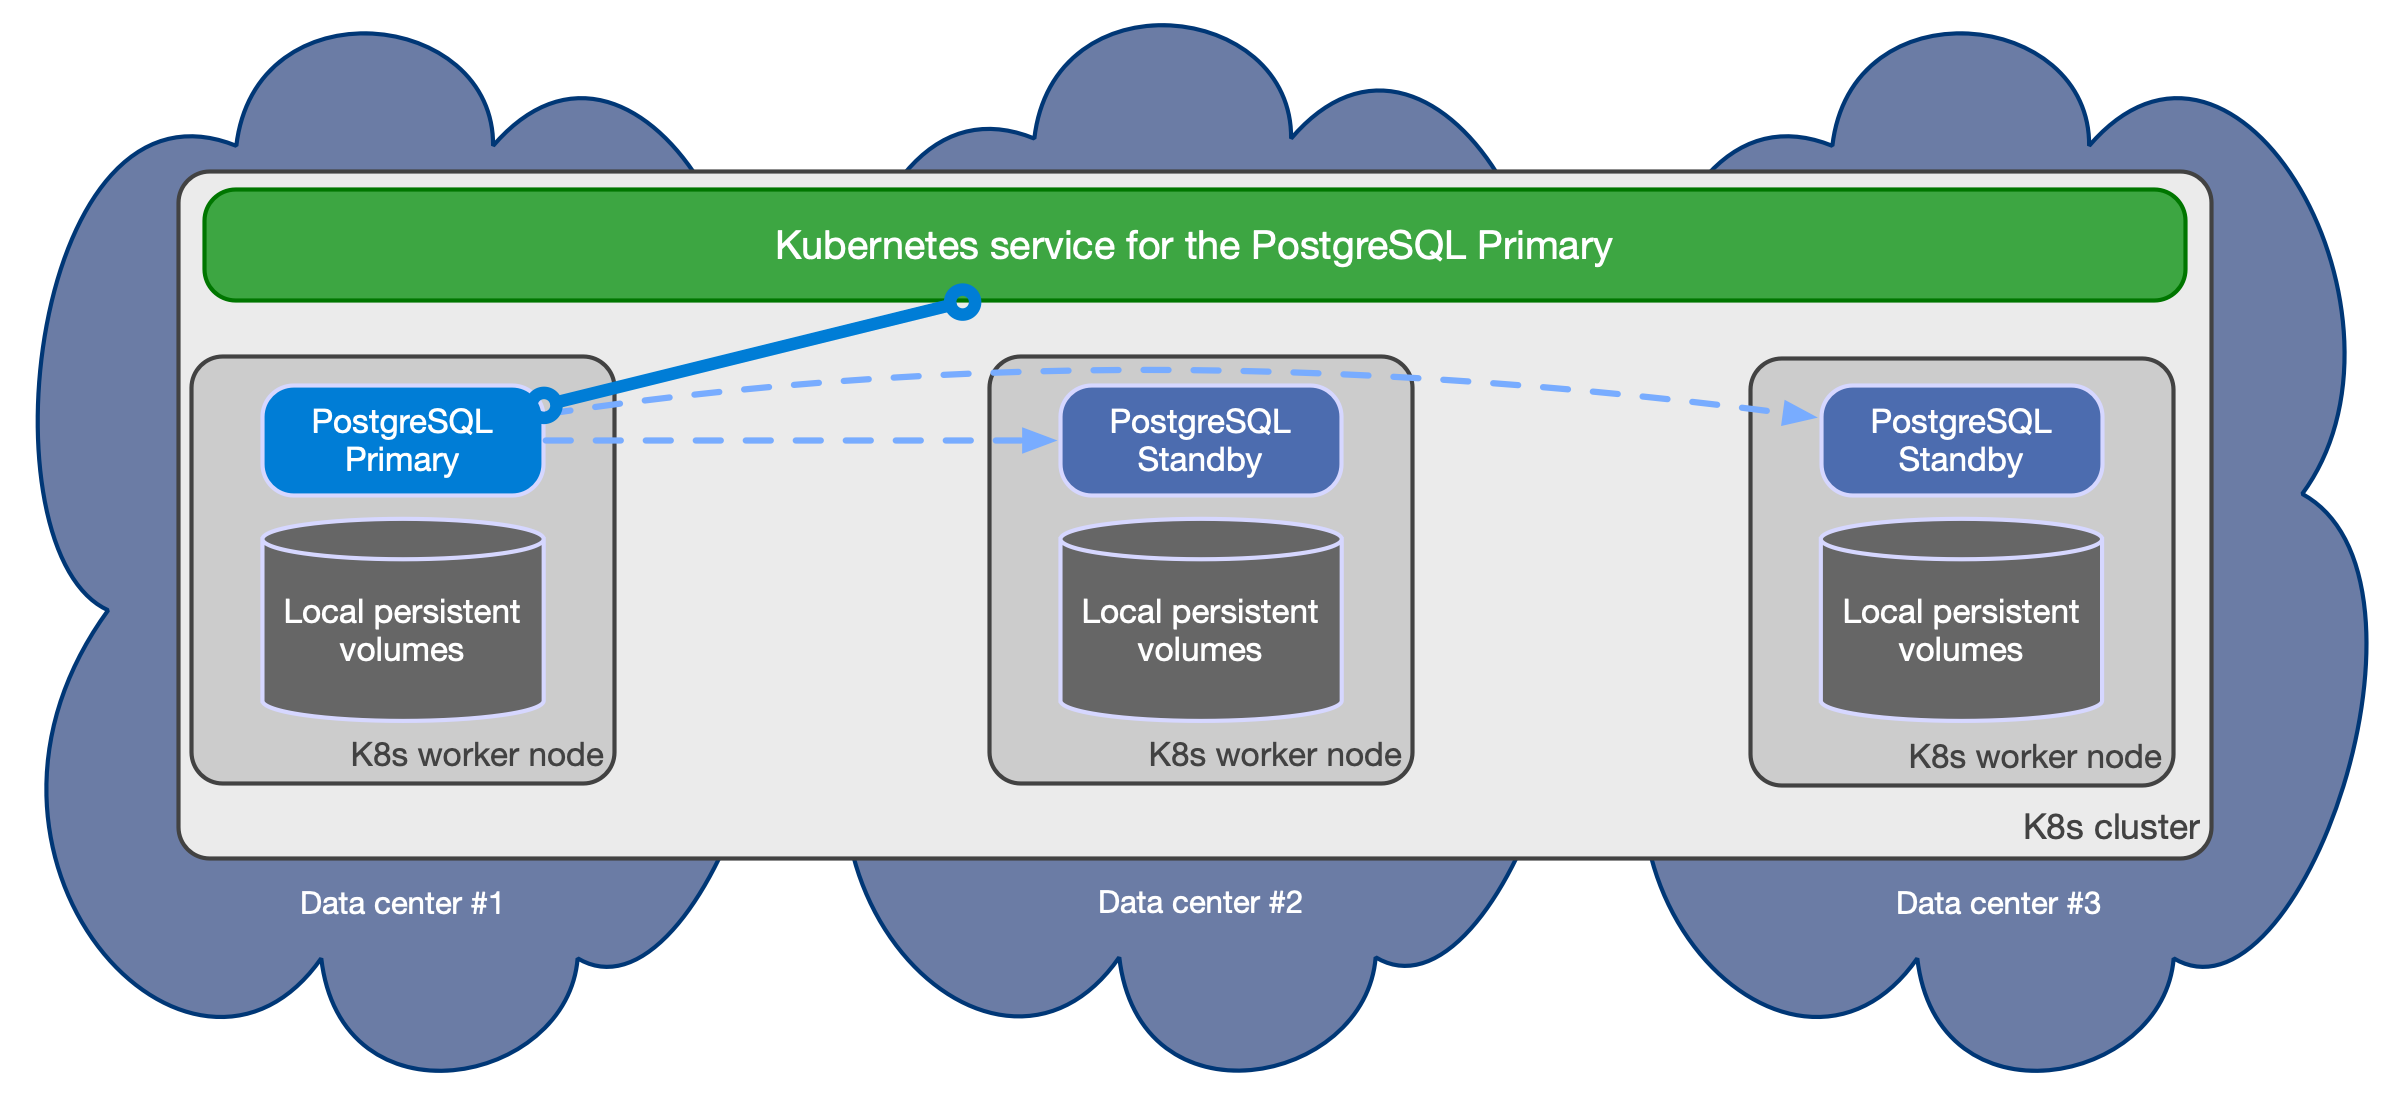
\includegraphics[width=0.75\linewidth]{source/implementation/evaluation/postgresql_ha_solutions/cloudnativepg/k8s-pg-architecture}
        \caption{CloudNativePG - Kubernetes - PostgreSQL}
        \label{fig:k8s-pg-architecture}
    \end{figure}
\end{flushleft}
\begin{flushleft}
    Dabei werden die read-write workloads an den primären Node gesendet:
    \begin{figure}[H]
        \centering
        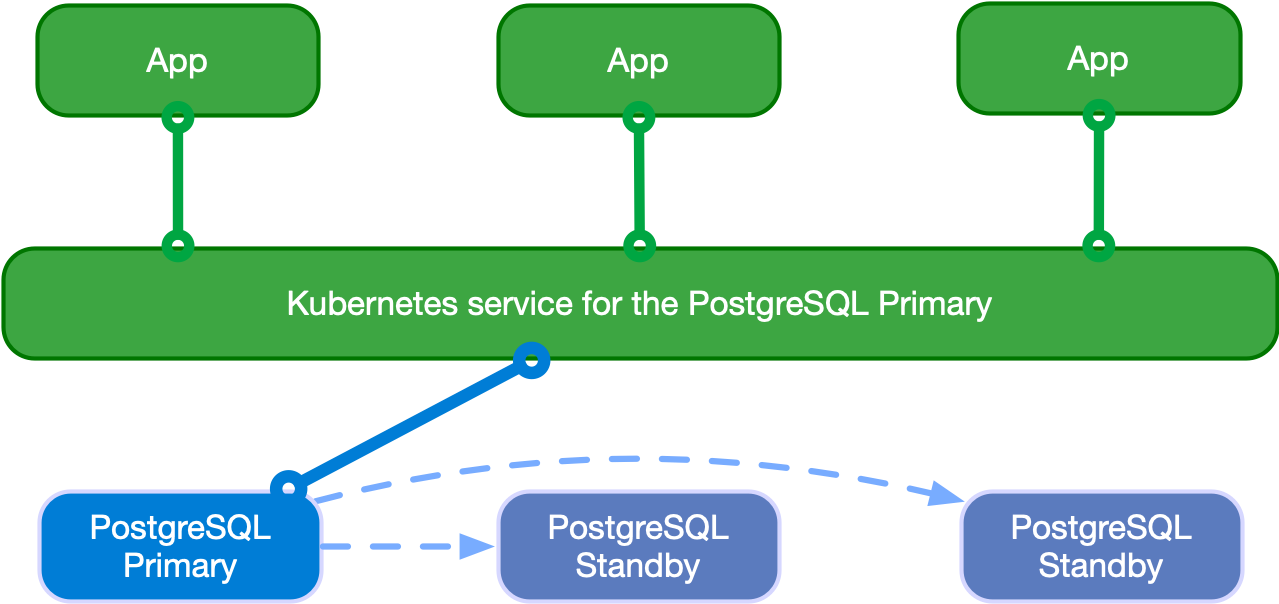
\includegraphics[width=0.75\linewidth]{source/implementation/evaluation/postgresql_ha_solutions/cloudnativepg/cloudnativepg-architecture-rw}
        \caption{CloudNativePG - Kubernetes - Read-write workloads}
        \label{fig:cloudnativepg-architecture-rw}
    \end{figure}
\end{flushleft}
\clearpage
\begin{flushleft}
    Read-only workloads werden per round robin an die Replikas zugewiesen:
    \begin{figure}[H]
        \centering
        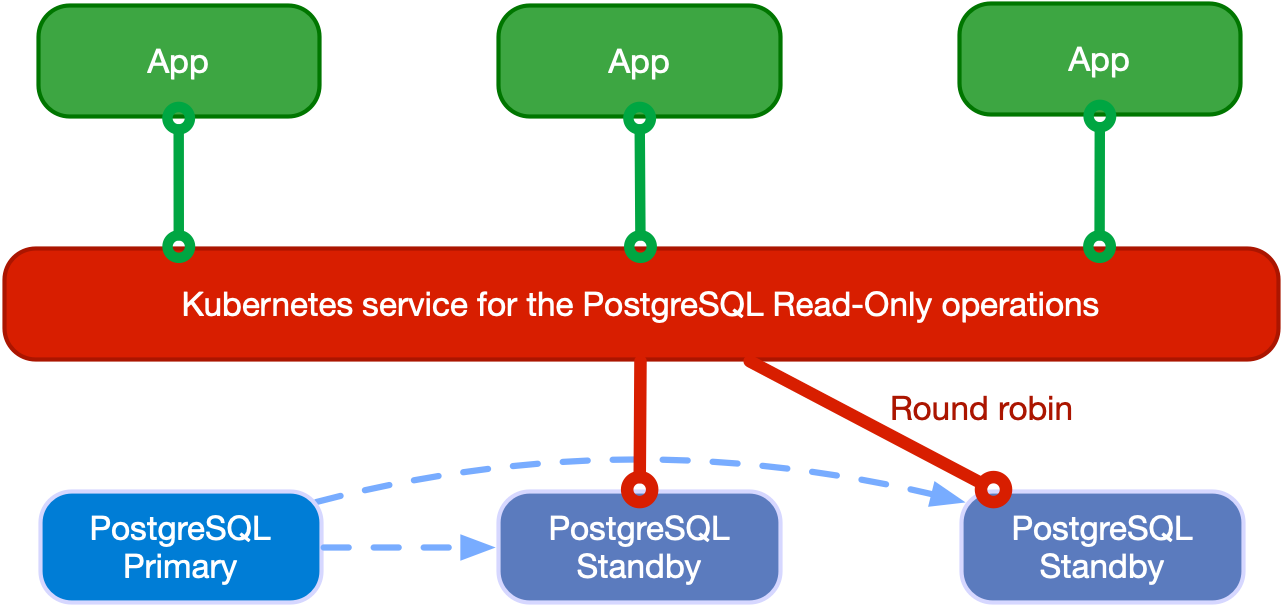
\includegraphics[width=0.75\linewidth]{source/implementation/evaluation/postgresql_ha_solutions/cloudnativepg/cloudnativepg-architecture-read-only}
        \caption{CloudNativePG - Kubernetes - Read-only workloads}
        \label{fig:cloudnativepg-architecture-read-only}
    \end{figure}
\end{flushleft}
\begin{flushleft}
    Es könnten auch Lösungen mit Designated Kubernetes-Clustern in einem anderen RZ oder einer anderen Geo-Region realisiert werden.
\end{flushleft}
\begin{flushleft}
    \paragraph{Maintenance}
    Das Projekt hat viele offene Issues.\\
    Der Code wird aber gut gepflegt, nicht mehr verwendeter Code wird auch regelmässig entfernt.\\
    Hin und wieder müssen grössere Aufräumaktionen gestartet, zudem finden die Commits immer am Monatsende statt.\\
    Dafür erfüllt das Projekt die meisten Community Standards.\\
    Die Vollständige Dokumentation ist im \hyperref[subsec:maintenance_cloudnativepg]{Anhang - Maintenance} zu finden.
\end{flushleft}
\begin{flushleft}
    \paragraph{Synergien und Mehrwert}
    CloudNativePG bleibt ein monolithisches System, welches aber keine Möglichkeit bietet, auch auf einem normalen Serversetting betrieben zu werden.
\end{flushleft}
\begin{flushleft}
    Daher bietet CloudNativePG weder einen Benefit durch seine Architektur noch mit der Möglichkeit,\\Synergien nutzen zu können.
\end{flushleft}